% Opcje klasy 'iithesis' opisane sa w komentarzach w pliku klasy. Za ich pomoca
% ustawia sie przede wszystkim jezyk oraz rodzaj (lic/inz/mgr) pracy.
\documentclass[shortabstract]{iithesis}
\usepackage{amssymb}
\usepackage{float}

\usepackage{tikz-uml}
%\usepackage[utf8]{inputenc}

%%%%% DANE DO STRONY TYTUŁOWEJ
% Niezaleznie od jezyka pracy wybranego w opcjach klasy, tytul i streszczenie
% pracy nalezy podac zarowno w jezyku polskim, jak i angielskim.
% Pamietaj o madrym (zgodnym z logicznym rozbiorem zdania oraz estetyka) recznym
% zlamaniu wierszy w temacie pracy, zwlaszcza tego w jezyku pracy. Uzyj do tego
% polecenia \fmlinebreak.
\polishtitle    {Aplikacja webowa wspomagająca zarządzanie\fmlinebreak pracownikami obsługi widowni teatru}
\englishtitle   {Web Application Supporting the Management of Theater Audience Service Staff}
\polishabstract{
W pracy inżynierskiej przedstawiono proces projektowania i implementacji aplikacji webowej do zarządzania pracą bileterów i koordynatorów w Teatrze Muzycznym Capitol. Aplikacja została zaprojektowana w celu usprawnienia procesów organizacyjnych, umożliwiającym pracownikom łatwe zgłaszanie dyspozycyjności, przeglądanie grafików pracy oraz raportowanie czasu pracy. Koordynatorzy uzyskali narzędzie do efektywnej alokacji zasobów ludzkich i zarządzania wydarzeniami teatralnymi. System wykorzystuje technologie takie, jak: Spring Boot, Hibernate, baza danych H2, Thymeleaf oraz Bootstrap, a jego architektura oparta jest na Domain-Driven Design. W ramach testowania zaimplementowano testy jednostkowe przy użyciu JUnit i Mockito. Aplikacja została pozytywnie oceniona przez pracowników teatru, którzy wskazali również kierunki jej dalszego rozwoju takie, jak: rozbudowa statystyk o pracownikach, stworzenie aplikacji mobilnej oraz systemu powiadomień. Praca stanowi podstawę do dalszego rozwoju systemu, który może być dostosowany do przyszłych wymagań i wyzwań teatru.
}

\englishabstract{
This engineering thesis presents the design and implementation process of a web application for managing the work of ticket agents and coordinators at the Capitol Musical Theater. The application was designed to streamline organizational processes, enabling employees to easily report availability, review work schedules, and report working hours. Coordinators gained a tool for efficient human resource allocation and management of theatrical events. The system employs technologies such as Spring Boot, Hibernate, H2 database, Thymeleaf, and Bootstrap, and its architecture is based on Domain-Driven Design. Unit tests were implemented using JUnit and Mockito for testing purposes. The application received positive feedback from theater staff, who also indicated directions for its further development, such as expanding employee statistics, creating a mobile application, and a notification system. The thesis lays the foundation for the further development of the system, which can be adapted to meet future requirements and challenges of the theater.
}
% w pracach wielu autorow nazwiska mozna oddzielic poleceniem \and
\author         {Adam Jarząbek}
% w przypadku kilku promotorow, lub koniecznosci podania ich afiliacji, linie
% w ponizszym poleceniu mozna zlamac poleceniem \fmlinebreak
\advisor        {dr inż. Leszek Grocholski}
\date          {14 czerwca 2024}                     % Data zlozenia pracy
% Dane do oswiadczenia o autorskim wykonaniu
%\transcriptnum {}                     % Numer indeksu
%\advisorgen    {dr. Jana Kowalskiego} % Nazwisko promotora w dopelniaczu
%%%%%

%%%%% WLASNE DODATKOWE PAKIETY
%
\usepackage{graphicx,listings,amsmath,amssymb,amsthm,amsfonts,tikz}
%
%%%%% WŁASNE DEFINICJE I POLECENIA
%
%\theoremstyle{definition} \newtheorem{definition}{Definition}[chapter]
%\theoremstyle{remark} \newtheorem{remark}[definition]{Observation}
%\theoremstyle{plain} \newtheorem{theorem}[definition]{Theorem}
%\theoremstyle{plain} \newtheorem{lemma}[definition]{Lemma}
%\renewcommand \qedsymbol {\ensuremath{\square}}
% ...
%%%%%

\begin{document}

%%%%% POCZĄTEK ZASADNICZEGO TEKSTU PRACY

\chapter{Wprowadzenie}

\section{Opis problemu}

Teatry jako instytucje kultury odgrywają kluczową rolę w życiu społecznym, oferując widzom różnorodne formy rozrywki i edukacji. Jednak za kulisami efektywne funkcjonowanie takiego miejsca wymaga skomplikowanej organizacji pracy wielu osób. W Teatrze Muzycznym Capitol, gdzie autor pracy jest zatrudniony jako pracownik obsługi widowni, codzienne wyzwania związane z koordynacją pracy około 40 bileterów stanowią istotny problem operacyjny. Bileterzy pełnią różne funkcje:  od sprawdzania biletów, przez obsługę szatni, aż po pilnowanie porządku w trakcie spektakli. Zarządzanie ich pracą, ze względu na zmienną dyspozycyjność i różnorodność stanowisk, wymaga elastycznego podejścia i precyzyjnego planowania.

Do tej pory proces ten był realizowany za pomocą arkusza kalkulacyjnego Google Sheets oraz tradycyjnej papierowej dokumentacji. Taki sposób zarządzania, choć częściowo efektywny, posiada liczne ograniczenia. Brak centralizacji danych, trudności w szybkim dostępie do aktualnych informacji, ograniczone możliwości personalizacji oraz brak automatyzacji w przydzielaniu stanowisk to tylko niektóre z problemów, które autor zidentyfikował jako pracownik i obserwator.

W niniejszej pracy inżynierskiej postawiono sobie za cel stworzenie aplikacji webowej, która usprawni proces zarządzania pracownikami obsługi widowni w Teatrze Muzycznym Capitol. Aplikacja ta ma umożliwić pracownikom łatwe i intuicyjne zgłaszanie swojej dyspozycyjności, przeglądanie przydzielonych im wydarzeń i stanowisk oraz dostęp do kluczowych informacji o spektaklach i scenach. Z kolei dla kierownictwa teatru aplikacja ma oferować narzędzia do efektywnego zarządzania zasobami ludzkimi, w tym konfigurację scen, rodzajów stanowisk, tworzenie wydarzeń oraz automatyczne przydzielanie pracowników do zadań.


\section{Przegląd istniejących rozwiązań}

Przed opisem proponowanego rozwiązania warto przyjrzeć wadom i zaletom rozwiązania aktualnie używanego w teatrze oraz alternawnym rozwiązaniom komercyjnym.

\subsection{Arkusze Google Sheets}

\subsubsection{Opis rozwiązania}
Arkusze Google Sheets stanowią obecnie podstawowe narzędzie do zarządzania pracownikami obsługi widowni w Teatrze Muzycznym Capitol. Cały system oparty na arkuszach kalkulacyjnych składa się z kilku zintegrowanych zakładek, z których każda pełni określoną funkcję w procesie planowania pracy bileterów.

Pierwszą z nich jest zakładka ,,dyspozycyjność'', która ma postać tabeli z kolumną zawierającą imiona i nazwiska pracowników po lewej stronie. Każda kolejna kolumna odpowiada poszczególnym wydarzeniom, zawierając informacje takie, jak: data, nazwa spektaklu, godzina oraz scena. Pracownicy zaznaczają w tej tabeli swoją dyspozycyjność na dane wydarzenie, wpisując ,,tak'' w odpowiedniej komórce. Brak dyspozycyjności oznaczany jest poprzez wpisanie ,,nie''. Po upływie terminu na zaznaczanie dyspozycyjności kierownik ukrywa zakładkę ,,dyspozycyjność'' i tworzy nową zakładkę ,,zatwierdzone''.


\begin{figure}[h] % Opcja 'h' oznacza 'here', czyli umieszczenie obrazka w miejscu definicji
\centering % Wycentrowanie obrazka
\includegraphics[width=1.0\textwidth]{dyspo-sheets.png} % Wstawienie obrazka
\caption{Fragment akrusza do zaznaczania dyspozycyjności} % Podpis pod obrazkiem
\end{figure}


Arkusz ,,zatwierdzone'' ma podobny układ do arkusza ,,dyspozycyjność'', ale słowo ,,tak'' przy danym wydarzeniu i pracowniku oznacza, że pracownik został oficjalnie przydzielony do pracy na tym wydarzeniu. Zazwyczaj do jednego wydarzenia przypisywanych jest, w zależności od sceny, 17 lub 6 pracowników.

\begin{figure}[h] % Opcja 'h' oznacza 'here', czyli umieszczenie obrazka w miejscu definicji
\centering % Wycentrowanie obrazka
\includegraphics[width=1.0\textwidth]{zatwierdzone.png} % Wstawienie obrazka
\caption{Fragment akrusza ,,Zatwierdzone'' z częściowo przypisanymi stanowiskami} % Podpis pod obrazkiem
\label{fig:dyspo} % Etykieta do odwoływania się do obrazka w tekście
\end{figure}

Dodatkowo istnieje arkusz ,,Bileterzy'', który zawiera tabelę z imionami, nazwiskami oraz numerami telefonów pracowników i koordynatora. W miarę zbliżania się danego wydarzenia, w zakładce ,,zatwierdzone'', w komórkach z ,,tak'', dopisywane są konkretne stanowiska, na których pracownicy mają pełnić swoje obowiązki.

Raportowanie czasu pracy bileterów odbywa się poprzez fizyczną dokumentację uzupełnianą po każdym wydarzeniu.


\subsubsection{Wady i zalety}
Wady i zalety tego rozwiązania są następujące:

\textbf{Zalety:}
\begin{itemize}
  \item Dostępność – Arkusze Google Sheets są dostępne z każdego miejsca i na każdym urządzeniu z dostępem do internetu.
  \item Możliwości - dzięki wykorzystaniu Google Sheets kordynator może korzystać z dobrodziejstw arkuszy kalkulacyjnychtakich takich jak formuły i formatowanie warunkowe.
  \item Znajomość narzędzia – wielu użytkowników jest już zaznajomionych z obsługą arkuszy kalkulacyjnych, co obniża próg wejścia dla nowych pracowników.
\end{itemize}

\newpage

\textbf{Wady:}
\begin{itemize}
  \item Brak personalizacji – wszyscy pracownicy korzystają z tego samego widoku arkusza, co oznacza brak indywidualnych tabel do zarządzania własną dyspozycyjnością czy grafikiem pracy.
  \item Problemy z bezpieczeństwem – dostęp do arkusza mają wszystkie osoby, które posiadają link, co stwarza ryzyko nieautoryzowanego dostępu i manipulacji danymi.
  \item Brak automatyzacji – proces przydzielania zadań jest całkowicie manualny, co zwiększa ryzyko błędów i jest czasochłonne dla kierownictwa.
  \item Ryzyko utraty danych – błędne operacje użytkowników mogą prowadzić do przypadkowego usunięcia ważnych informacji bez możliwości łatwego odzyskania.
\end{itemize}


\subsection{When I Work}

\subsubsection{Opis rozwiązania}
When I Work to komercyjne oprogramowanie zaprojektowane do zarządzania grafikami pracy, które umożliwia pracownikom zgłaszanie swojej dyspozycyjności oraz umożliwia menedżerom szybkie tworzenie i modyfikowanie grafików pracy. Aplikacja oferuje możliwość komunikacji z pracownikami i posiada aplikację mobilną, co pozwala na łatwe zarządzanie zmianami w pracy z dowolnego miejsca.
\begin{figure}[h]
    \centering
    \includegraphics[width=1.0\linewidth]{wheniwork.jpg}
    \caption{Aplikacja do zarządania pracownikami When I Work}
    \label{fig:wiw}
\end{figure}



\subsubsection{Wady i zalety}

\textbf{Zalety:}
\begin{itemize}
  \item Intuicyjny interfejs użytkownika, który ułatwia zarządzanie grafikami pracy.
  \item Funkcja komunikacji w aplikacji pozwala na szybkie przekazywanie informacji między pracownikami a zarządem.
  \item Aplikacja mobilna umożliwia pracownikom łatwy dostęp do grafiku pracy i zgłaszanie dyspozycyjności w dowolnym miejscu i czasie.
  \item Automatyzacja procesu tworzenia grafiku może znacznie oszczędzić czas menedżerów i zwiększyć efektywność planowania.
\end{itemize}


\textbf{Wady:}
\begin{itemize}
  \item Koszt subskrypcji może być barierą dla mniejszych organizacji z ograniczonym budżetem.
  \item Wymagany czas na szkolenie pracowników w zakresie korzystania z nowego systemu.
  \item Brak dostosowania narzędzia do potrzeb teatru, czyli definiowania konkretnych spektakli i scen.
\end{itemize}

\section{Funkcje aplikacji}

Poniżej wymienionio wymagania funkcjonalne i niefunkcjonalne aplikacji. Zostały one sporządzone na podstawie doświadczeń autora w pracy w jednym z wrocławskich teatrów w roli biletera oraz na podstawie wywiadu zebranego wśród pracowników tej instytucji.

\subsection{Wymagania funkcjonalne}

Wymagania funkcjonalne zostały podzielone na trzy kategorie, w zależności od roli użytkownika w systemie: wymagania dla bileterów, wymagania dla koordynatorów oraz wymagania ogólne.


\newpage
\subsubsection*{Wymagania dla bileterów}
\begin{enumerate}
  \item Bileter może wyświetlać informacje kontaktowe innych pracowników.
  \item Bileter może wyświetlać informacje o spektaklach oraz o scenach, na których odbywają się wydarzenia.
  \item Bileter może wyświetlać wszystkie wydarzenia z podziałem na grupy wydarzeń (np. na miesiące).
  \item Bileter może wyświetlać informacje o wydarzeniach, do których jest przypisany, wraz z informacją o stanowisku pracy.
  \item Bileter może określać swoją dyspozycyjność na dane wydarzenia.
  \item Bileter może przeglądać informacje o wydarzeniach z obecnego tygodnia, do których jest przypisany.
  \item Bileter może raportować swój czas pracy oraz wyświetlać łączny czas pracy w danym miesiącu.
\end{enumerate}


\subsubsection*{Wymagania dla koordynatorów}
\begin{enumerate}
  \item Koordynator może tworzyć, usuwać i edytować konta użytkowników.
  \item Koordynator może określać jakie istnieją stanowiska pracy biletera oraz określać ich typ.
  \item Koordynator może tworzyć i edytować sceny, na których odbywają się spektakle, w tym określać, jakie i ile stanowisk trzeba obsadzić, aby obsłużyć wydarzenie odbywające się na tej scenie.
  \item Koordynator może tworzyć i edytować spektakle grane w teatrze.
  \item Koordynator może tworzyć i usuwać wydarzenia (spektakl + data i godzina) z podziałem na grupy.
  \item Koordynator może włączać i wyłączać możliwość uzupełniania dyspozycyjności dla danej grupy wydarzeń oraz sterować widocznością danych grup wydarzeń w grafiku.
  \item Koordynator może przypisywać pracowników do wydarzeń oraz przypisywać stanowiska do pracowników.
  \item Koordynator ma możliwość wyświetlania raportów pracy bileterów.
\end{enumerate}

\subsubsection*{Wymagania ogólne}
\begin{enumerate}
  \item Użytkownik może zalogować się do systemu, używając adresu e-mail oraz hasła.
  \item W zależności od przydzielonej roli użytkownik będzie miał dostęp do odpowiednich funkcjonalności. Przewidziane role: Bileter oraz Koordynator.
  \item Aplikacja ma umożliwiać automatyczne przypisanie stanowisk do pracowników w danej grupie wydarzeń według sensownej heurystyki.
\end{enumerate}


\subsection{Wymagania niefunkcjonalne}
System powinien spełniać następujące wymagania niefunkcjonalne:
\begin{enumerate}
  \item Czas odpowiedzi systemu na żądania użytkownika nie powinien przekraczać 2 sekund.
  \item Interfejs użytkownika powinien być intuicyjny i dostosowany do potrzeb użytkowników o różnym stopniu zaawansowania.
  \item Aplikacja powinna być dostępna na najpopularniejszych systemach operacyjnych i przeglądarkach internetowych, w tym na Windows, macOS, Linux, Chrome, Firefox, Safari i Edge w ich aktualnych wersjach.
  \item Wszelkie aktualizacje systemu powinny odbywać się z minimalnym wpływem na dostępność i wydajność systemu.
  \item Dokumentacja systemu powinna być kompletna, aktualna i łatwo dostępna dla użytkowników oraz administratorów systemu.
\end{enumerate}

\section{Wybrane przypadki użycia}

Poniżej przedstawiono kilka wybranych przypadków użycia, które ilustrują, jak aplikacja może być wykorzystywana przez różnych użytkowników w teatrze.

\subsection{Przypadek użycia dla biletera}

\begin{itemize}
  \item \textbf{Sprawdzenie grafiku pracy:} bileter loguje się do systemu i wyświetla swoje nadchodzące wydarzenia oraz przypisane stanowiska pracy.
  \item \textbf{Deklaracja dyspozycyjności:} bileter aktualizuje swoją dyspozycyjność w systemie, określając, na które wydarzenia może się zgłosić.
  \item \textbf{Raportowanie czasu pracy:} bileter po zakończeniu pracy raportuje czas pracy w systemie i przegląda łączny czas pracy w danym miesiącu.
\end{itemize}

\subsection{Przypadek użycia dla koordynatora}

\begin{itemize}
  \item \textbf{Zarządzanie kontami użytkowników:} koordynator tworzy, edytuje lub usuwa konta użytkowników, dostosowując uprawnienia do roli w teatrze.
  \item \textbf{Organizacja wydarzeń:} koordynator tworzy nowe wydarzenia, określa potrzebne stanowiska pracy i przypisuje pracowników.
  \item \textbf{Przypisanie stanowisk:} koordynator używa funkcji automatycznego przypisywania stanowisk, aby optymalnie rozplanować zasoby ludzkie.
\end{itemize}

\subsection{Przypadek użycia ogólny}

\begin{itemize}
  \item \textbf{Logowanie i dostęp do funkcji:} Użytkownik loguje się do systemu i korzysta z funkcji dostępnych dla swojej roli – biletera lub koordynatora.
\end{itemize}

\subsection{Diagram UML wybranych przypadków użycia}

Poniżej przedstawiono diagram UML, który zawiera dwa aktorów: Biletera i Koordynatora, oraz siedem przypadków użycia. Przypadki użycia "Logowanie i dostęp do funkcji" jest wspólny dla obu aktorów i jest dziedziczony przez wszystkie inne przypadki użycia, co jest przedstawione na diagramie poprzez linie dziedziczenia.

\begin{tikzpicture}
  % Define the actors
  \umlactor[x=-7, y=0]{Bileter}
  \umlactor[x=7, y=0]{Koordynator}

  % Define the use cases for Bileter
  \umlusecase[x=-3, y=2, width=2.5cm, name=usecase1]{Sprawdzenie grafiku pracy}
  \umlusecase[x=-3, y=0, width=2.5cm, name=usecase2]{Deklaracja dyspozycyjności}
  \umlusecase[x=-3, y=-2, width=2.5cm, name=usecase3]{Raportowanie czasu pracy}

  % Define the use cases for Koordynator
  \umlusecase[x=3, y=2, width=2.5cm, name=usecase4]{Zarządzanie kontami użytkowników}
  \umlusecase[x=3, y=0, width=2.5cm, name=usecase5]{Organizacja wydarzeń}
  \umlusecase[x=3, y=-2, width=2.5cm, name=usecase6]{Przypisanie stanowisk}

  % Define the general use case
  \umlusecase[x=0, y=-4, width=2.5cm, name=usecase7]{Logowanie i zmiana hasła}

  % Associate actors with use cases
  \umlassoc{Bileter}{usecase1}
  \umlassoc{Bileter}{usecase2}
  \umlassoc{Bileter}{usecase3}
  \umlassoc{Koordynator}{usecase4}
  \umlassoc{Koordynator}{usecase5}
  \umlassoc{Koordynator}{usecase6}

  % Associate general use case with specific ones
  \umlinherit[geometry=|-|]{usecase7}{usecase1}
  \umlinherit[geometry=|-|]{usecase7}{usecase2}
  \umlinherit[geometry=|-|]{usecase7}{usecase3}
  \umlinherit[geometry=|-|]{usecase7}{usecase4}
  \umlinherit[geometry=|-|]{usecase7}{usecase5}
  \umlinherit[geometry=|-|]{usecase7}{usecase6}

\caption{Diagram UML wybranych przypadków użycia}

\end{tikzpicture}

\chapter{Napotkane problemy i ich rozwiązania}

W tym rozdziale przedstawione zostaną kluczowe rozwiązania i osiągnięcia, które udało mi się zrealizować podczas pracy nad projektem. Opisane zostaną innowacje i usprawnienia, które przyczyniają się do zwiększenia efektywności i użytkowości aplikacji.

\section{Łatwo dostępna aplikacja z prostym interfejsem}

Jednym z głównych celów projektu było stworzenie aplikacji, która będzie łatwo dostępna i intuicyjna w obsłudze dla wszystkich użytkowników. Z tego względu kładziono duży nacisk na prostotę interfejsu użytkownika, co pozwoliło na szybką adaptację nawet dla osób, które nie mają doświadczenia w pracy z podobnymi systemami. Użycie nowoczesnych technologii webowych takich jak Thymeleaf oraz Bootstrap pozwoliło na stworzenie klarownego i responsywnego designu, który jest dostosowany do różnych urządzeń i rozmiarów ekranów.

\section{Uniwersalna aplikacja dla różnych ról użytkowników}

Dzięki zastosowaniu Spring Security w połączeniu z Thymeleaf udało się stworzyć uniwersalne rozwiązanie, które serwuje odpowiednie treści w zależności od roli i uprawnień zalogowanego użytkownika. Taki model pozwolił na stworzenie jednej aplikacji, która dynamicznie dostosowuje dostępne opcje i funkcjonalności, zarówno dla bileterów, jak i koordynatorów. To rozwiązanie znacznie upraszcza zarządzanie systemem i redukuje potrzebę tworzenia oddzielnych interfejsów dla różnych grup użytkowników.

\section{Wysoka konfigurowalność aplikacji}

Kolejnym istotnym aspektem projektu jest wysoka konfigurowalność aplikacji. Zaimplementowane mechanizmy pozwalają na elastyczne zarządzanie scenami, spektaklami, stanowiskami pracy, a także na podział na różne grupy wydarzeń. Taka konstrukcja systemu daje możliwość definiowania zróżnicowanych grafików, co jest szczególnie przydatne w przypadku organizacji dodatkowych wydarzeń, takich jak festiwale czy przeglądy. Łatwość konfiguracji jest również nieoceniona w sytuacji wprowadzania do repertuaru nowych spektakli, a także w przypadku obsługiwania wydarzeń w innych lokalizacjach.

\section{Automatyczne przypisywanie stanowisk}

Koordynatorzy często stają przed wyzwaniem sprawiedliwego i efektywnego przydzielania stanowisk pracownikom. Opracowany algorytm automatycznego przypisywania stanowisk stanowi odpowiedź na ten problem, umożliwiając przejrzystą organizację pracy oraz uwzględnienie indywidualnej historii zadań każdego pracownika.

\subsection{Proces przydziału}

Proces przydziału rozpoczyna się od wyczyszczenia poprzednich przypisań stanowisk, co umożliwia adaptację do aktualnych potrzeb wydarzenia. Dla każdej imprezy w grupie algorytm sortuje wymagane stanowiska według ich priorytetu, zapewniając obsadzanie kluczowych ról w pierwszej kolejności.

\subsection{Heurystyka wyboru pracownika}

Algorytm wybiera najbardziej odpowiedniego pracownika dla danego stanowiska, kierując się
heurystyką, która uwzględnia liczbę poprzednich przydziałów do określonego typu stanowiska
oraz czas, który upłynął od ostatniego obsadzenia stanowiska przez danego pracownika. Taki system rotacji zapobiega monotonii pracy i sprzyja równomiernemu rozwojowi umiejętności wśród personelu.


\section{Rozszerzalność aplikacji}

Aplikacja została zbudowana z myślą o łatwej rozbudowie. Modułowa architektura i zastosowanie Spring Boot pozwalają na sprawną integrację nowych funkcji i usprawnień, co przygotowuje system na przyszłe wymagania użytkowników.

\chapter{Podręcznik użytkownika}

W niniejszym rozdziale przedstawiono instrukcję obsługi aplikacji, zarówno dla bileterów, jak i koordynatorów. Wersja aplikacji dostępna dla użytkownika jest determinowana przez rolę przypisaną do jego konta.

\section{Dostęp do aplikacji}

Aplikacja do zarządzania pracą w Teatrze Muzycznym Capitol jest dostępna online oraz może być uruchomiona lokalnie. Poniżej przedstawiono instrukcje dotyczące obu metod dostępu.

\subsection{Dostęp online}

Aplikacja jest dostępna w wersji demonstracyjnej pod adresem internetowym: \url{https://capitol-manager.onrender.com}. Aby się zalogować, należy użyć następujących danych testowych:

\begin{itemize}
  \item Konto biletera:
  \begin{itemize}
    \item Email: bileter@przyklad.pl
    \item Hasło: capitol
  \end{itemize}
  \item Konto koordynatora:
  \begin{itemize}
    \item Email: koordynator@przyklad.pl
    \item Hasło: capitol
  \end{itemize}
\end{itemize}

Przy korzystaniu z wersji demonstracyjnej aplikacji online czasy odpowiedzi mogą być wyższe ze względu na wykorzystanie darmowych usług hostingowych.

\subsection{Uruchomienie lokalne}

Aplikacja Capitol Manager została zaprojektowana do łatwego uruchamiania lokalnego za pomocą pliku JAR, który automatycznie inicjalizuje bazę danych H2 w pamięci. Aby uruchomić aplikację lokalnie, należy wykonać następujące polecenie w terminalu:

\begin{verbatim}
java -jar capitol-manager-1.jar
\end{verbatim}

Po uruchomieniu aplikacji należy otworzyć przeglądarkę internetową i wpisać adres \texttt{http://localhost:8080}. Aplikacja powinna być teraz dostępna i gotowa do użycia z danymi testowymi załadowanymi do bazy danych.

\section{Instrukcja obsługi – część ogólna}

\subsection{Strona główna}

Ekran główny prezentuje listę wydarzeń, do których przypisany jest użytkownik, zaplanowanych
na bieżący tydzień. Aby zapoznać się ze szczegółami wydarzenia, w tym z przypisanym stanowiskiem, wystarczy kliknąć na etykietę reprezentującą dane wydarzenie.

Poniżej wyświetlana jest lista nadchodzących zmian oraz kalendarz z wydarzeniami przypisanymi do użytkownika w danym miesiącu.

\begin{figure}[h]
    \centering
    \includegraphics[width=\linewidth]{ekran_glowny_bileter.png}
    \caption{Ekran główny serwisu}
    \label{fig:glowny}
\end{figure}

\subsection{Nawigacja}
Pasek nawigacyjny umieszczony na górze każdej strony, umożliwia szybkie przełączanie się między poszczególnymi sekcjami aplikacji.

\subsection{Wylogowanie i zmiana hasła}
Aby wylogować się z konta, należy skorzystać z opcji \textit{Moje konto} $\rightarrow$ \textit{Wyloguj} w pasku nawigacyjnym. W celu zmiany hasła użytkownik powinien wybrać \textit{Moje konto} $\rightarrow$ \textit{Zmień hasło}.


\section{Instrukcja obsługi – część dla bileterów}

\subsection{Wyświetlanie informacji o pracownikach}

Dane o pracownikach zarejestrowanych w systemie dostępne są w sekcji \textit{Pracownicy}. Sekcja ta zawiera imiona, nazwiska oraz numery telefonów pracowników z wyróżnionymi na początku listy koordynatorami.

\begin{figure}[h]
    \centering
    \includegraphics[width=\linewidth]{user-list.png}
    \caption{Lista pracowników z wyróżnionymi koordynatorami.}
    \label{fig:user-list}
\end{figure}


\subsection{Wyświetlanie informacji o scenach i spektaklach}

\subsubsection{Sceny}
\label{stages}
W sekcji \textit{Informacje} $\rightarrow$ \textit{Sceny} znajduje się tabela z danymi dotyczącymi wszystkich scen, w tym nazwy scen, liczby miejsc siedzących oraz adresy.

\begin{figure}[h]
    \centering
    \includegraphics[width=\linewidth]{stage-list.png}
    \caption{Lista scen.}
    \label{fig:stage-list}
\end{figure}

\subsubsection{Spektakle}
Dane dotyczące repertuaru teatru dostępne są w sekcji \textit{Informacje} $\rightarrow$ \textit{Spektakle}, gdzie dla każdego spektaklu podane są tytuł, scena, czas trwania oraz dodatkowe informacje.

\begin{figure}[h]
    \centering
    \includegraphics[width=\linewidth]{show-list.png}
    \caption{Lista spektakli.}
    \label{fig:show-list}
\end{figure}



\subsection{Grafiki}

Sekcja \textit{Grafik} prezentuje aktywne grupy wydarzeń. Dla grup z dostępnym grafikiem można go wyświetlić, wybierając \textit{Pokaż wydarzenia}. Wyświetlana jest także liczba zmian przypisanych do użytkownika w ramach danej grupy.
\newpage
W przypadku możliwości zgłoszenia dyspozycyjności dla danej grupy wydarzeń, użytkownik może to uczynić, klikając \textit{Wypełnij dyspozycyjność}. Na kafelku grupy wyświetlany jest stopień wypełnienia dyspozycyjności oraz procentowa dyspozycyjność, czyli odsetek wydarzeń, na które użytkownik zaznaczył swój udział.

\begin{figure}[h]
    \centering
    \includegraphics[width=\linewidth]{grupy_wydarzen.png}
    \caption{Grupy wydarzeń z możliwością wyświetlenia lub wypełnienia dyspozycyjności.}
    \label{fig:event-groups}
\end{figure}

\subsection{Zaznaczanie dyspozycyjności}

Wybór opcji \textit{Zaznacz dyspozycyjność} otwiera widok kalendarza, na którym można zaznaczyć dostępność dla wydarzeń z wybranej grupy. Informacje o każdym wydarzeniu obejmują tytuł spektaklu, scenę, godzinę rozpoczęcia oraz czas trwania. Wybór dyspozycyjności ,,Tak'' lub ,,Nie'' jest automatycznie zapisywany po jego dokonaniu.

\begin{figure}[H]
    \centering
    \includegraphics[width=\linewidth]{dyspo.png}
    \caption{Ekran zaznaczania dyspozycyjności z oznaczonymi na zielono dostępnymi wydarzeniami.}
    \label{fig:availability}
\end{figure}

\subsection{Wyświetlanie grafiku}

Po wybraniu \textit{Pokaż wydarzenia} prezentowany jest kalendarz z wydarzeniami należącymi do danej grupy, zawierającymi tytuł spektaklu, nazwę sceny, godzinę rozpoczęcia, czas trwania oraz przypisane stanowisko (jeśli zostało przydzielone).

Wydarzenia, do których użytkownik został oficjalnie przypisany, są wyróżnione kolorem zielonym.

\begin{figure}[H]
    \centering
    \includegraphics[width=\linewidth]{grafik.png}
    \caption{Kalendarz z wydarzeniami grupy, z zaznaczonymi przypisanymi wydarzeniami.}
    \label{fig:schedule}
\end{figure}



\subsection{Raportowanie czasu pracy}

Aby zaraportować czas pracy po zmianie, należy wybrać \textit{Raportowanie czasu pracy} z paska nawigacyjnego.

Możliwe jest wyświetlenie listy raportów z wybranego miesiąca oraz podsumowania przepracowanych godzin. Wybór miesiąca odbywa się poprzez wybranie nazwy miesiąca i roku, a następnie kliknięcie \textit{Filtruj}. Usunięcie raportu możliwe jest po użyciu przycisku \textit{Usuń}.

\begin{figure}[h]
    \centering
    \includegraphics[width=\linewidth]{payroll.png}
    \caption{Lista raportów czasu pracy z danego miesiąca.}
    \label{fig:payroll}
\end{figure}

Aby utworzyć nowy raport, należy wybrać \textit{Utwórz}. W kolejnym kroku określa się datę, godzinę rozpoczęcia i zakończenia zmiany (z dokładnością do 15 minut), a zatwierdzenie odbywa się poprzez kliknięcie \textit{Zatwierdź}.


\newpage

\section{Instrukcja obsługi – część dla koordynatora}

\subsection{Lista pracowników}
\label{user-list}

Wyświetlenie listy użytkowników możliwe jest po wybraniu \textit{Pracownicy} z menu. Prezentowana jest tabela zawierająca dane koordynatorów i bileterów.

\begin{figure}[h]
    \centering
    \includegraphics[width=\linewidth]{user-list-manager.png}
    \caption{Lista pracowników dostępna dla koordynatora.}
    \label{fig:user-list-manager}
\end{figure}

\subsection{Edycja i tworzenie kont pracowników}

\subsubsection{Tworzenie nowego konta}

Aby stworzyć konto pracownika, należy kliknąć \textit{Utwórz} na widoku \nameref{user-list}, a następnie podać adres e-mail, imię, nazwisko, numer telefonu oraz przypisać jedną z dwóch ról.

Konto jest tworzone po wciśnięciu \textit{Zapisz}, a domyślne hasło dla nowego konta to \textit{capitol}.

\begin{figure}[h]
    \centering
    \includegraphics[width=\linewidth]{user-edit.png}
    \caption{Formularz tworzenia nowego konta pracownika.}
    \label{fig:user-edit}
\end{figure}

\subsubsection{Edycja konta}

Edycja danych pracownika odbywa się po kliknięciu \textit{Edytuj} przy jego danych na widoku \nameref{user-list} i zapisaniu zmian przyciskiem \textit{Zapisz}.

\subsection{Wyświetlanie raportów pracy}

Aby wyświetlić raporty godzin pracy dla danego pracownika, należy wybrać opcję \textit{Raporty czasu pracy} na widoku listowym pracowników.

\subsection{Konfiguracja scen}
\label{stage-edit}

Lista scen, na których odbywają się spektakle, jest dostępna po wybraniu \textit{Konfiguracja} $\rightarrow$ \textit{Sceny}. Z tego miejsca można przejść do tworzenia nowej sceny, edycji istniejącej sceny oraz zarządzania stanowiskami.

\begin{figure}[h]
    \centering
    \includegraphics[width=\linewidth]{stage-list-manager.png}
    \caption{Lista scen dostępna dla koordynatora.}
    \label{fig:stage-list-manager}
\end{figure}

\subsubsection{Tworzenie nowej sceny}
Aby dodać nową scenę, wybiera się \textit{Utwórz} na widoku listowym scen, a następnie podaje nazwę sceny, liczbę miejsc oraz adres. Po zapisaniu sceny można przejść do edycji stanowisk.

\subsubsection{Edycja sceny}
Edycja sceny możliwa jest po wybraniu \textit{Edytuj} przy wybranej scenie. Z poziomu edycji można również usunąć scenę lub przejść do edycji stanowisk. Usunięcie sceny jest zablokowane, jeśli scena jest przypisana do spektaklu.

\begin{figure}[h]
    \centering
    \includegraphics[width=\linewidth]{stage-edit.png}
    \caption{Formularz edycji sceny.}
    \label{fig:stage-edit}
\end{figure}

\subsection{Konfiguracja stanowisk}

Stanowiska określają liczbę pracowników potrzebnych do obsługi wydarzenia i są przypisywane do scen. Aby skonfigurować stanowiska dla sceny, wybiera się \textit{Edytuj stanowiska} na widoku listy scen lub edycji sceny.

\begin{figure}[h]
    \centering
    \includegraphics[width=\linewidth]{position-edit.png}
    \caption{Edycja stanowisk dla konkretnej sceny.}
    \label{fig:position-edit}
\end{figure}

Edycja stanowisk umożliwia dodawanie i modyfikowanie stanowisk dla sceny. W modalu edycji określa się nazwę stanowiska, typ oraz liczbę potrzebnych pracowników.


\subsection{Konfiguracja spektakli}
\label{show-edit}

Konfiguracja spektakli jest dostępna po wybraniu opcji \textit{Konfiguracja} $\rightarrow$ \textit{Spektakle} z menu.

\subsubsection{Tworzenie i edycja spektakli}

Tworzenie nowego spektaklu lub edycja istniejącego odbywa się z widoku listy spektakli. W formularzu edycyjnym podaje się tytuł spektaklu, czas trwania, scenę oraz dodatkowe informacje.

\newpage

\subsection{Konfiguracja wydarzeń}

W tej sekcji opisano kroki konieczne do zaplanowania i zarządzania harmonogramem wydarzeń.

\subsubsection{Grupy wydarzeń}
Dostęp do grup wydarzeń umożliwia opcja \textit{Grafik} w menu.

Aby utworzyć nową grupę wydarzeń, należy skorzystać z przycisku \textit{+}. Aby zmienić nazwę grupy wydarzeń, należy kliknąć na tę nazwę i wprowadzić nową w ukazanym oknie modalnym.

\begin{figure}[h]
    \centering
    \includegraphics[width=1\linewidth]{grupy.png}
    \caption{Ekran do zarządzania grupami wydarzeń}
    \label{fig:grupy}
\end{figure}

\subsubsection{Tworzenie wydarzeń}

Tworzenie nowych wydarzeń rozpoczyna się od wyboru \textit{Edytuj wydarzenia} w ramach wybranej grupy wydarzeń.

Na ekranie ukazują się wydarzenia podzielone na tygodnie. Nawigacja między tygodniami odbywa się za pomocą przycisków po lewej i prawej stronie ekranu.

Aby dodać wydarzenie, wystarczy najechać kursorem na konkretny dzień i wybrać \textit{Dodaj wydarzenie}. W otwierającym się oknie modalnym należy określić spektakl (zobacz: \nameref{show-edit}), datę i godzinę rozpoczęcia wydarzenia.

Edycja lub usunięcie wydarzenia jest możliwa po najechaniu na nie kursorem i wybraniu odpowiedniej ikony.

\begin{figure}[h]
    \centering
    \includegraphics[width=1\linewidth]{event-list.png}
    \caption{Formularz umożliwiający konfigurowanie wydarzeń}
    \label{fig:event-list}
\end{figure}

\subsubsection{Aktywowanie dyspozycyjności}

Aby umożliwić użytkownikom wypełnienie dyspozycyjności dla danej grupy wydarzeń, należy zaznaczyć pole wyboru \textit{Pokaż dyspozycyjność}. Po zakończonym okresie zgłaszania dyspozycyjności pole to powinno zostać odznaczone, aby zapobiec dalszemu korzystaniu z tej funkcji przez bileterów.

\begin{figure}[h]
    \centering
    \includegraphics[width=1\linewidth]{av-actice.png}
    \caption{Przełącznik umożliwiający włączenie lub wyłączenie funkcji wypełniania dyspozyzyjności}
    \label{fig:av-active}
\end{figure}

\subsubsection{Przypisywanie pracowników do wydarzeń}

Po zebraniu informacji o dyspozycyjności bileterów, przystępuje się do przypisywania ich do wydarzeń. W tym celu wybiera się \textit{Przypisz pracowników} w odpowiedniej grupie wydarzeń.

W interfejsie przypisywania pracowników znajduje się tabela, gdzie po lewej stronie wymienieni są pracownicy, a w kolumnach przedstawione są wydarzenia. Przypisanie biletera do wydarzenia odbywa się poprzez zaznaczenie pola wyboru w odpowiedniej komórce tabeli. Nieaktywne pola wyboru wskazują na niedyspozycyjność biletera w danym dniu.

W ostatniej kolumnie tabeli znajdują się informacja o liczbie wydarzeń przypisanych do biletera w stosunku do jego dyspozycyjności.

Wydarzenia, do których przypisano wystarczającą liczbę bileterów, są oznaczone kolorem zielonym, a te wymagające jeszcze przypisania – kolorem czerwonym.

Wydarzenia są podzielone na strony. Aby przełączać si między stronami, należy skorzystać z przycisków \textit{Poprzednia strona} i \textit{Następna strona}.

\begin{figure}[h]
    \centering
    \includegraphics[width=1\linewidth]{assign-users.png}
    \caption{Widok przypisywania pracowników do wydarzeń}
    \label{fig:enter-label}
\end{figure}

\subsubsection{Aktywowanie grafiku}

Aby przypisania stały się widoczne dla bileterów, konieczne jest zaznaczenie opcji \textit{Pokazuj grafik}.

\begin{figure}[h]
    \centering
    \includegraphics[width=1\linewidth]{toggle-schedule-act.png}
    \caption{Przełącznik do sterowania widocznością wydarzeń z danej grupy}
    \label{fig:enter-label}
\end{figure}


\subsubsection{Przypisywanie stanowisk do pracowników}

Przydzielenie stanowisk dla bileterów na poszczególne wydarzenia rozpoczyna się od wyboru opcji \textit{Przypisz stanowiska}. Następnie, w odpowiedniej komórce tabeli, z listy rozwijanej wybiera się stanowisko, które ma być przypisane do pracownika.

\subsubsection{Automatyczne przypisywanie stanowisk}

Aplikacja posiada funkcję automatycznego przypisywania stanowisk. Aby z niej skorzystać, należy zaznaczyć wydarzenia, dla których stanowiska mają zostać przydzielone, a następnie kliknąć przycisk \textit{Automatycznie przypisz stanowiska dla zaznaczonych wydarzeń}.

\textit{Uwaga!} Użycie opcji automatycznego przypisywania stanowisk spowoduje nadpisanie wszystkich dotychczasowych przypisań dla zaznaczonych wydarzeń.

\begin{figure}[H]
    \centering
    \includegraphics[width=1\linewidth]{position-assign.png}
    \caption{Przypisywanie stanowisk do pracowników}
    \label{fig:enter-label}
\end{figure}

\subsubsection{Archiwizowanie wydarzeń}

Aby wydarzenia i grafik przestały być widoczne dla bileterów, lecz nadal można było przeglądać statystyki dotyczące danej grupy wydarzeń, należy odznaczyć oba pola wyboru: \textit{Pokazuj grafik} i \textit{Pokaż dyspozycyjność}.

Usuwanie grupy wydarzeń wraz z wszystkimi powiązanymi z nią wydarzeniami i przypisaniami odbywa się poprzez kliknięcie przycisku z ikoną kosza na śmieci.

\chapter{Część dla programistów}

Rozdział ten poświęcony jest omówieniu rozwiązań technicznych zastosowanych w trakcie tworzenia aplikacji.

\section{Kod aplikacji}

Kod aplikacji jest dostępny w publicznym repozytorium GitHub: \url{https://github.com/adamj00/capitol-manager}

\section{Architektura aplikacji}

Aplikacja została zaprojektowana z wykorzystaniem architektury wzorowanej na Domain-Driven Design, co pozwoliło na skoncentrowanie się na modelu domenowym oraz logiczne oddzielenie poszczególnych części systemu. DDD pozwala na efektywną współpracę między zespołem technicznym a ekspertami domenowymi, co jest kluczowe dla zrozumienia i rozwiązywania rzeczywistych problemów biznesowych.

\subsection{Domain-Driven Design}

Domain-Driven Design (DDD) to podejście do projektowania oprogramowania, które kładzie nacisk na zrozumienie modelu domenowego oraz jego efektywne odwzorowanie w kodzie aplikacji. Koncepcja DDD zakłada, że logika biznesowa jest kluczowym elementem oprogramowania i powinna być punktem centralnym w procesie projektowania systemu informatycznego.
\newpage
Model domenowy w DDD jest bogatym modelem, który zawiera zarówno elementy strukturalne, takie jak encje i obiekty wartości, jak i behawioralne, takie jak usługi, wydarzenia domenowe i agregaty. DDD promuje również głębokie zrozumienie domeny poprzez bliską współpracę z ekspertami biznesowymi, co pozwala na tworzenie oprogramowania, które dokładnie odpowiada potrzebom i zasadom danej dziedziny.

Architektura aplikacji oparta na DDD jest podzielona na cztery główne warstwy:

\begin{itemize}
    \item \textbf{Warstwa prezentacji} – odpowiedzialna za interakcję z użytkownikiem, prezentująca dane i przyjmująca od niego polecenia.
    \item \textbf{Warstwa aplikacyjna} – definiuje przepływ operacji w aplikacji, koordynuje działania i deleguje zadania do warstwy domenowej.
    \item \textbf{Warstwa domenowa} – serce aplikacji, gdzie zaimplementowana jest logika biznesowa i znajduje się model domenowy.
    \item \textbf{Warstwa infrastruktury} – zapewnia wsparcie techniczne dla pozostałych warstw, takie jak bazy danych, systemy komunikacji czy operacje wejścia/wyjścia.
\end{itemize}

Implementacja DDD wymaga stosowania odpowiednich wzorców projektowych, które pomagają w organizacji kodu i zarządzaniu złożonymi modelami domenowymi. Dzięki temu podejściu możliwe jest tworzenie skalowalnych, elastycznych i łatwych w utrzymaniu systemów informatycznych, które są ściśle dopasowane do specyfiki biznesowej.

\newpage

\section{Schemat bazy danych}
\label{schema}
Schemat bazy danych został opracowany w oparciu o model domenowy aplikacji i obejmuje 9 powiązanych ze sobą tabel.

\begin{figure}[H]
    \centering
    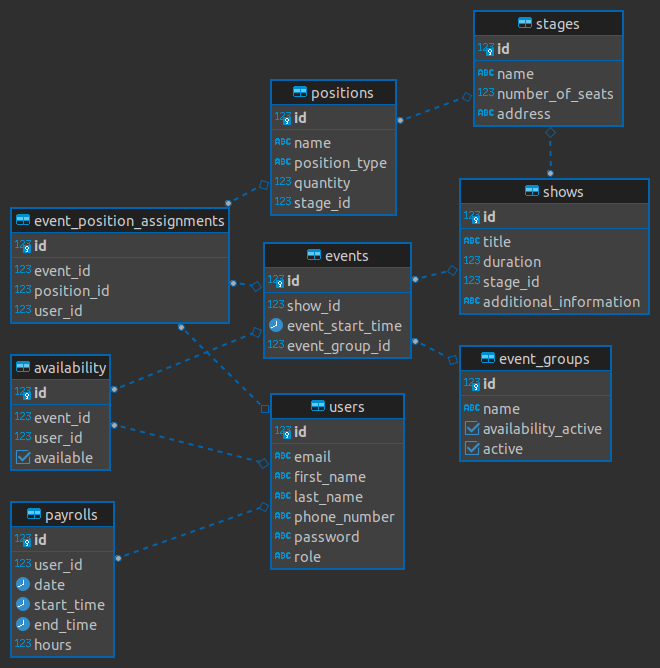
\includegraphics[width=0.8\linewidth]{schema.png}
    \caption{Schemat bazy danych.}
    \label{fig:chema}
\end{figure}

\section{Użyte technologie}

\subsection{Spring Boot}
Spring Boot jest narzędziem ułatwiającym tworzenie aplikacji w oparciu o platformę Spring, które zapewnia automatyczną konfigurację i zarządzanie zależnościami. Dzięki zastosowaniu \textit{inversion of control} (IoC) oraz \textit{dependency injection} (DI), Spring Boot umożliwia łatwe i szybkie tworzenie aplikacji gotowych do produkcji. Moduł Spring Security, używany wraz z Spring Boot, oferuje funkcjonalności związane z uwierzytelnianiem i autoryzacją\cite{springboot}.

\subsection{Hibernate}
Hibernate to biblioteka mapowania obiektowo-relacyjnego (ORM) dla języka Java, która ułatwia zarządzanie relacyjnymi bazami danych. Pozwala ona na odwzorowanie modelu obiektowego aplikacji na schemat bazy danych, co znacznie upraszcza operacje bazodanowe\cite{hibernate}.

\subsection{Baza danych H2}
H2 to lekka baza danych w pamięci, która jest idealna do szybkiego prototypowania i testowania aplikacji. Ze względu na prostotę w konfiguracji i możliwość ładowania początkowych danych, jest często wybierana do wersji demonstracyjnych aplikacji\cite{h2database}.

\subsection{Thymeleaf}
Thymeleaf to silnik szablonów HTML zaprojektowany dla aplikacji webowych w języku Java. Umożliwia tworzenie interaktywnych widoków, które mogą być łatwo zintegrowane z logiką aplikacji backendowej\cite{thymeleaf}.

\subsection{Bootstrap}
Bootstrap to framework CSS, który pomaga w szybkim projektowaniu responsywnych i atrakcyjnych interfejsów użytkownika. Oferuje zestaw narzędzi do stylizacji i komponentów interfejsu, które są łatwe do zaimplementowania\cite{bootstrap}.

\section{Testowanie}

W ramach projektu przygotowano testy jednostkowe dla niektórych serwisów aplikacyjnych oraz walidatorów. Testy jednostkowe są niezbędne do weryfikacji poprawności działania poszczególnych komponentów aplikacji poprzez izolowanie ich od reszty systemu.

\subsection{JUnit}

JUnit jest jednym z najpopularniejszych frameworków do pisania testów jednostkowych w języku Java. Pozwala on na szybkie i efektywne tworzenie testów, które mogą być automatycznie uruchamiane i sprawdzane pod kątem poprawności działania kodu. Framework JUnit dostarcza zestaw adnotacji pozwalających określać metody testowe, a także asercje do weryfikacji oczekiwanych wyników.


\newapge

JUnit jest nieoceniony w procesie ciągłej integracji i ciągłego dostarczania oprogramowania, ponieważ umożliwia łatwe włączenie testów jednostkowych do procesu budowania i wdrażania aplikacji\cite{junit}.

\subsection{Mockito}

Mockito to popularny framework do tworzenia i zarządzania obiektami zastępczymi (ang. "mocks") w testach jednostkowych dla języka Java. Umożliwia on izolację testowanego kodu od zależności zewnętrznych, co pozwala na przeprowadzanie testów w kontrolowanym środowisku. Mockito jest cenione za prostotę w tworzeniu obiektów zastępczych, łatwość weryfikacji zachowań oraz możliwość symulowania skomplikowanych interakcji między obiektami\cite{mockito}.

\chapter{Podsumowanie}

\section{Informacja zwrotna od pracowników teatru}

Po zaprezentowaniu systemu pracownikom teatru muzycznego Capitol zebrano cenne opinie, które pozwoliły ocenić funkcjonalność i potencjalne korzyści płynące z jego zastosowania. Bileterzy wyrazili entuzjazm, doceniając szczególnie łatwość w sprawdzaniu i zarządzaniu swoim grafikiem pracy. Możliwość deklarowania dyspozycyjności oraz raportowania czasu pracy w prosty i intuicyjny sposób została uznana za znaczące usprawnienie ich codziennych obowiązków.

Koordynatorzy również pozytywnie ocenili zaprezentowany system, zwracając uwagę na funkcję automatycznego przypisywania stanowisk, która znacznie ułatwia zarządzanie zasobami ludzkimi. Intuicyjne zarządzanie kontami użytkowników i wydarzeniami pozwala na efektywną organizację pracy, co przekłada się na oszczędność czasu i zwiększenie produktywności.

Choć ogólne wrażenia były bardzo pozytywne, użytkownicy zasugerowali kilka obszarów do dalszego rozwoju. Wśród rekomendacji znalazły się: rozbudowa statystyk o pracownikach, udoskonalenie interfejsu do przypisywania pracowników do wydarzeń oraz optymalizacja aplikacji pod kątem urządzeń mobilnych, co zapewniłoby jeszcze lepszą dostępność i wygodę korzystania z systemu.


\newpage

\section{Możliwości rozwoju aplikacji}

W oparciu o zebrane informacje zwrotne oraz własne analizy zidentyfikowano kilka kluczowych
obszarów, w których aplikacja mogłaby zostać rozwinięta. Do najbardziej obiecujących należą:

\begin{itemize}
  \item \textbf{Wyświetlanie statystyk o pracownikach:} rozbudowa funkcjonalności analitycznych, które pozwolą koordynatorom na lepsze planowanie pracy i ocenę wydajności pracowników.
  \item \textbf{Stworzenie API i aplikacji mobilnej:} dzięki temu bileterzy mogliby jeszcze łatwiej przeglądać zmiany i wypełniać dyspozycyjność, a koordynatorzy mieliby stały dostęp do systemu z poziomu urządzenia mobilnego.
  \item \textbf{System powiadomień:} automatyczne przypomnienia o nadchodzących zmianach lub konieczności wypełnienia dyspozycyjności mogłyby zwiększyć komunikację i efektywność działania całego teatru.
\end{itemize}

\section{Zakończenie}

Projekt aplikacji do zarządzania pracą w Teatrze Muzycznym Capitol zakończył się sukcesem. Prezentacja aplikacji użytkownikom spotkała się z pozytywnym przyjęciem, a jej funkcjonalności zostały wysoko ocenione przez bileterów i koordynatorów. Uzyskane informacje zwrotne stanowią solidną podstawę do dalszego rozwoju systemu. Przewidziane ulepszenia i nowe funkcje, takie jak rozbudowane statystyki o pracownikach czy aplikacja mobilna, mają potencjał do dalszego zwiększania efektywności i poprawy organizacji pracy. Perspektywa rozwoju aplikacji oraz jej skalowalność gwarantują sprostanie przyszłym wyzwaniom i potrzebom teatru.

%%%%% BIBLIOGRAFIA

\begin{thebibliography}{8}
\bibitem{springboot}
Spring Boot, \url{https://spring.io/projects/spring-boot}, dostęp 6 czerwca 2024.

\bibitem{springsecurity}
Spring Security, \url{https://spring.io/projects/spring-security}, dostęp 6 czerwca 2024.

\bibitem{hibernate}
Hibernate, \url{https://hibernate.org/orm/documentation/}, dostęp 6 czerwca 2024.

\bibitem{h2database}
H2 Database Engine, \url{http://www.h2database.com/}, dostęp 6 czerwca 2024.

\bibitem{thymeleaf}
Thymeleaf, \url{https://www.thymeleaf.org/documentation.html}, dostęp 6 czerwca 2024.

\bibitem{bootstrap}
Bootstrap, \url{https://getbootstrap.com/}, dostęp 6 czerwca 2024.

\bibitem{junit}
JUnit 5, \url{https://junit.org/junit5/}, dostęp 6 czerwca 2024.

\bibitem{mockito}
Mockito, \url{https://site.mockito.org/}, dostęp 6 czerwca 2024.

\end{thebibliography}

\end{document}
